\singlespacing
\chapter{This is chapter 2}
\label{ch2}
\doublespacing
\chaptermark{Chapter 2: This is.... }

\section{Introduction}
\label{sec: intro}

The chapter 2 consists of .....

\newpage

\begin{landscape}
\section{Figures}
\label{sec: figures}

\begin{figure}[!h]
\centering
  \caption{This is Figure 1}
    \label{fig: maps1}
    
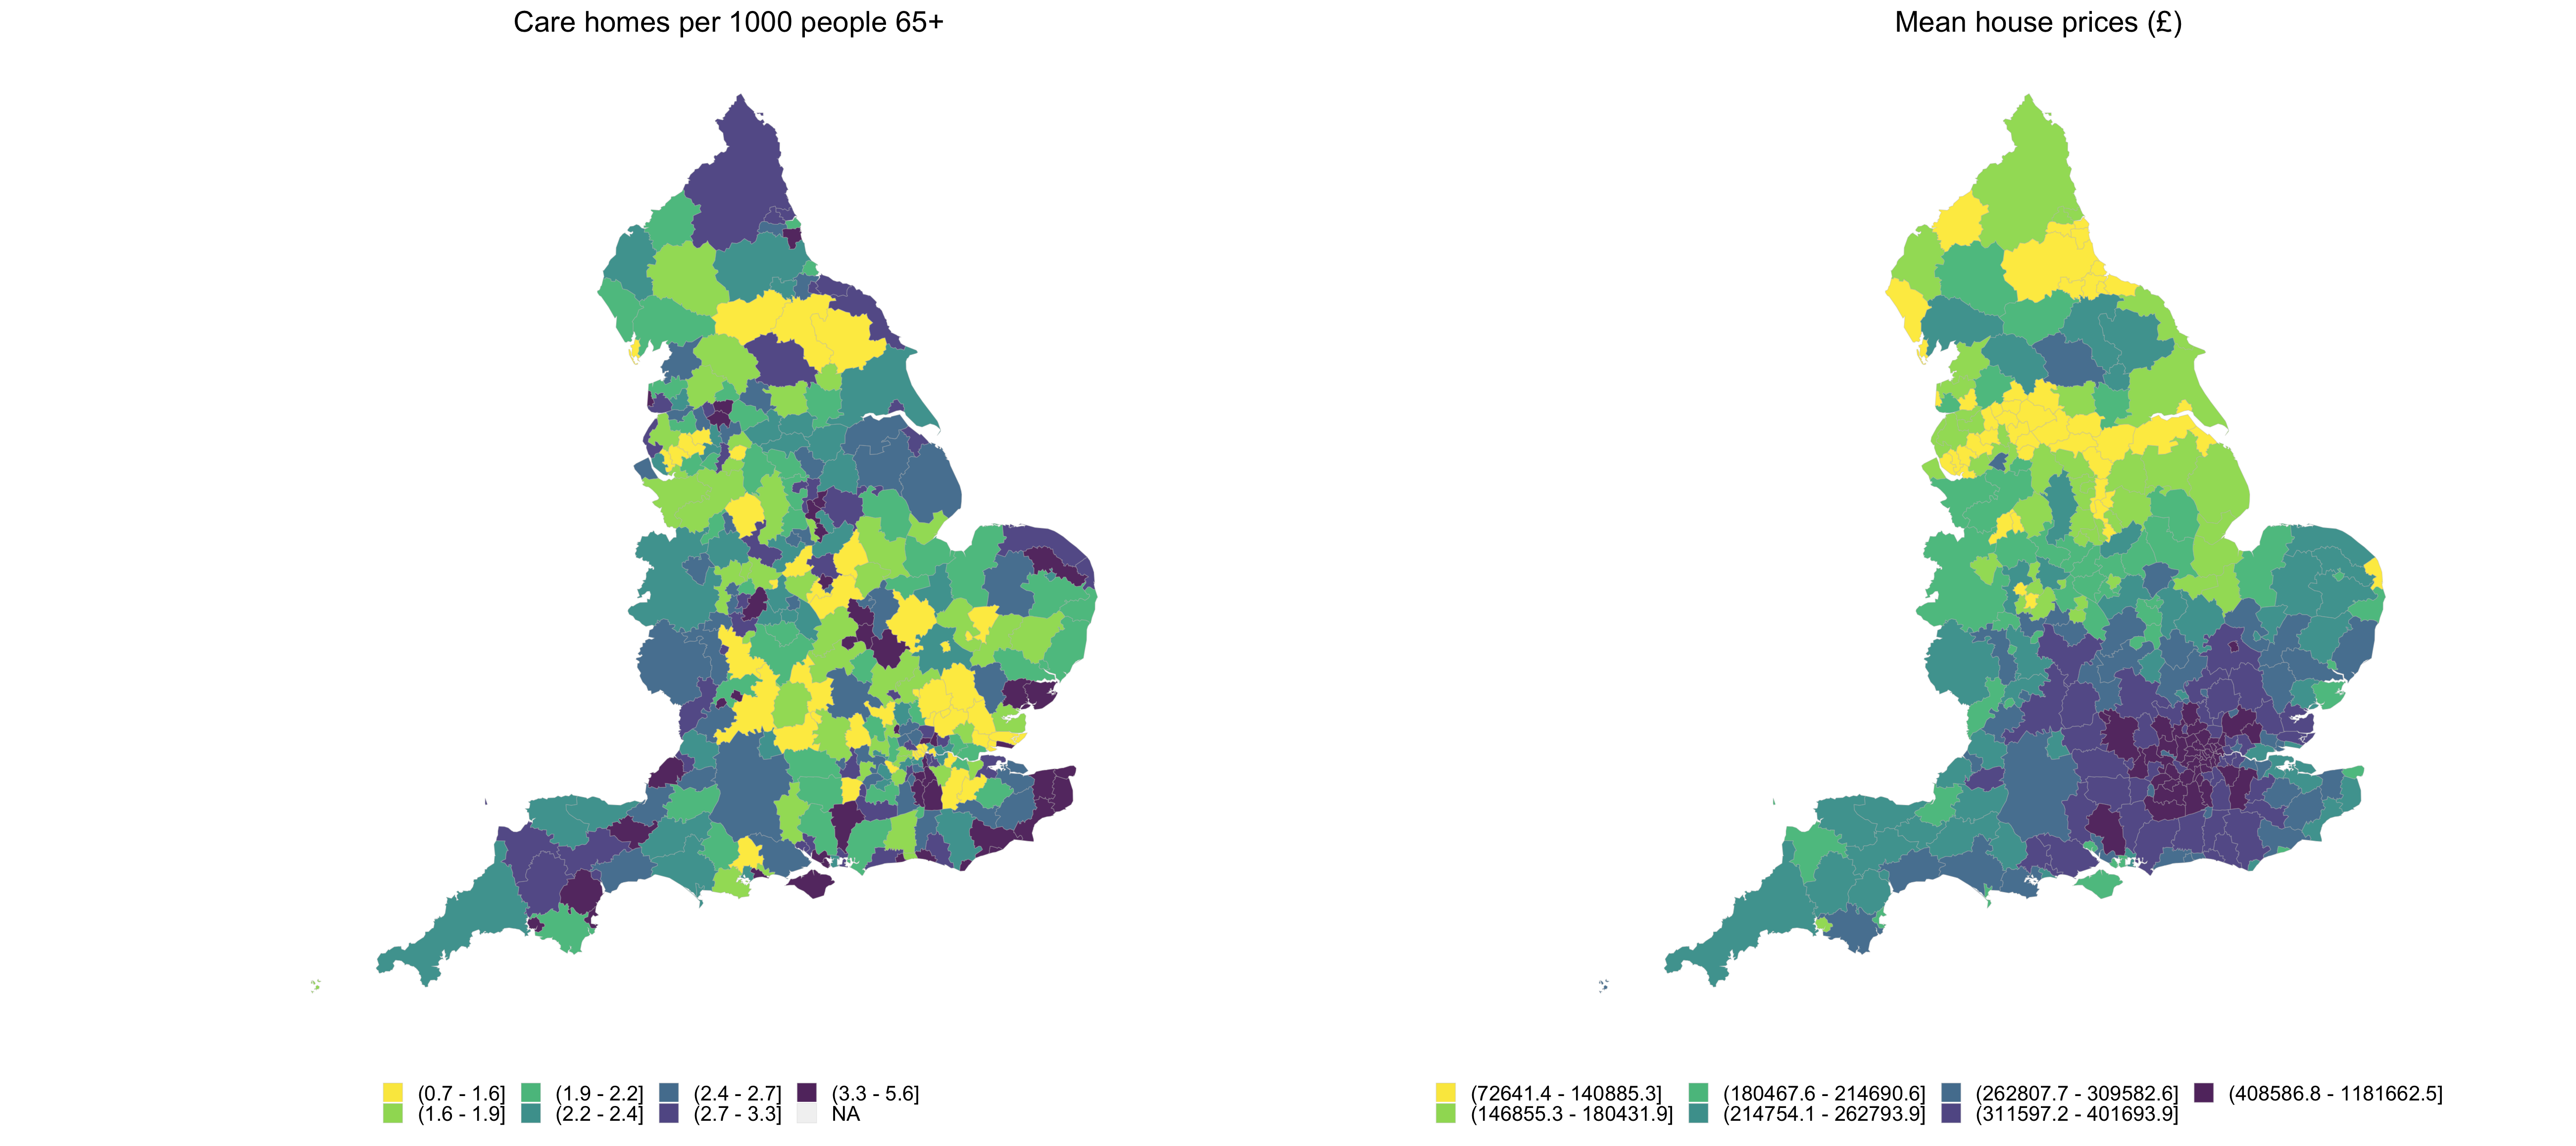
\includegraphics[width=1\textwidth]{ch_2/maps_test.png}


\floatfoot{{\textbf{Note}}: English districts.}
\end{figure}

\end{landscape}

\newpage 

\begin{figure}[!h]
\centering
  \caption{This is figure 2}
    \label{fig: maps2}
    
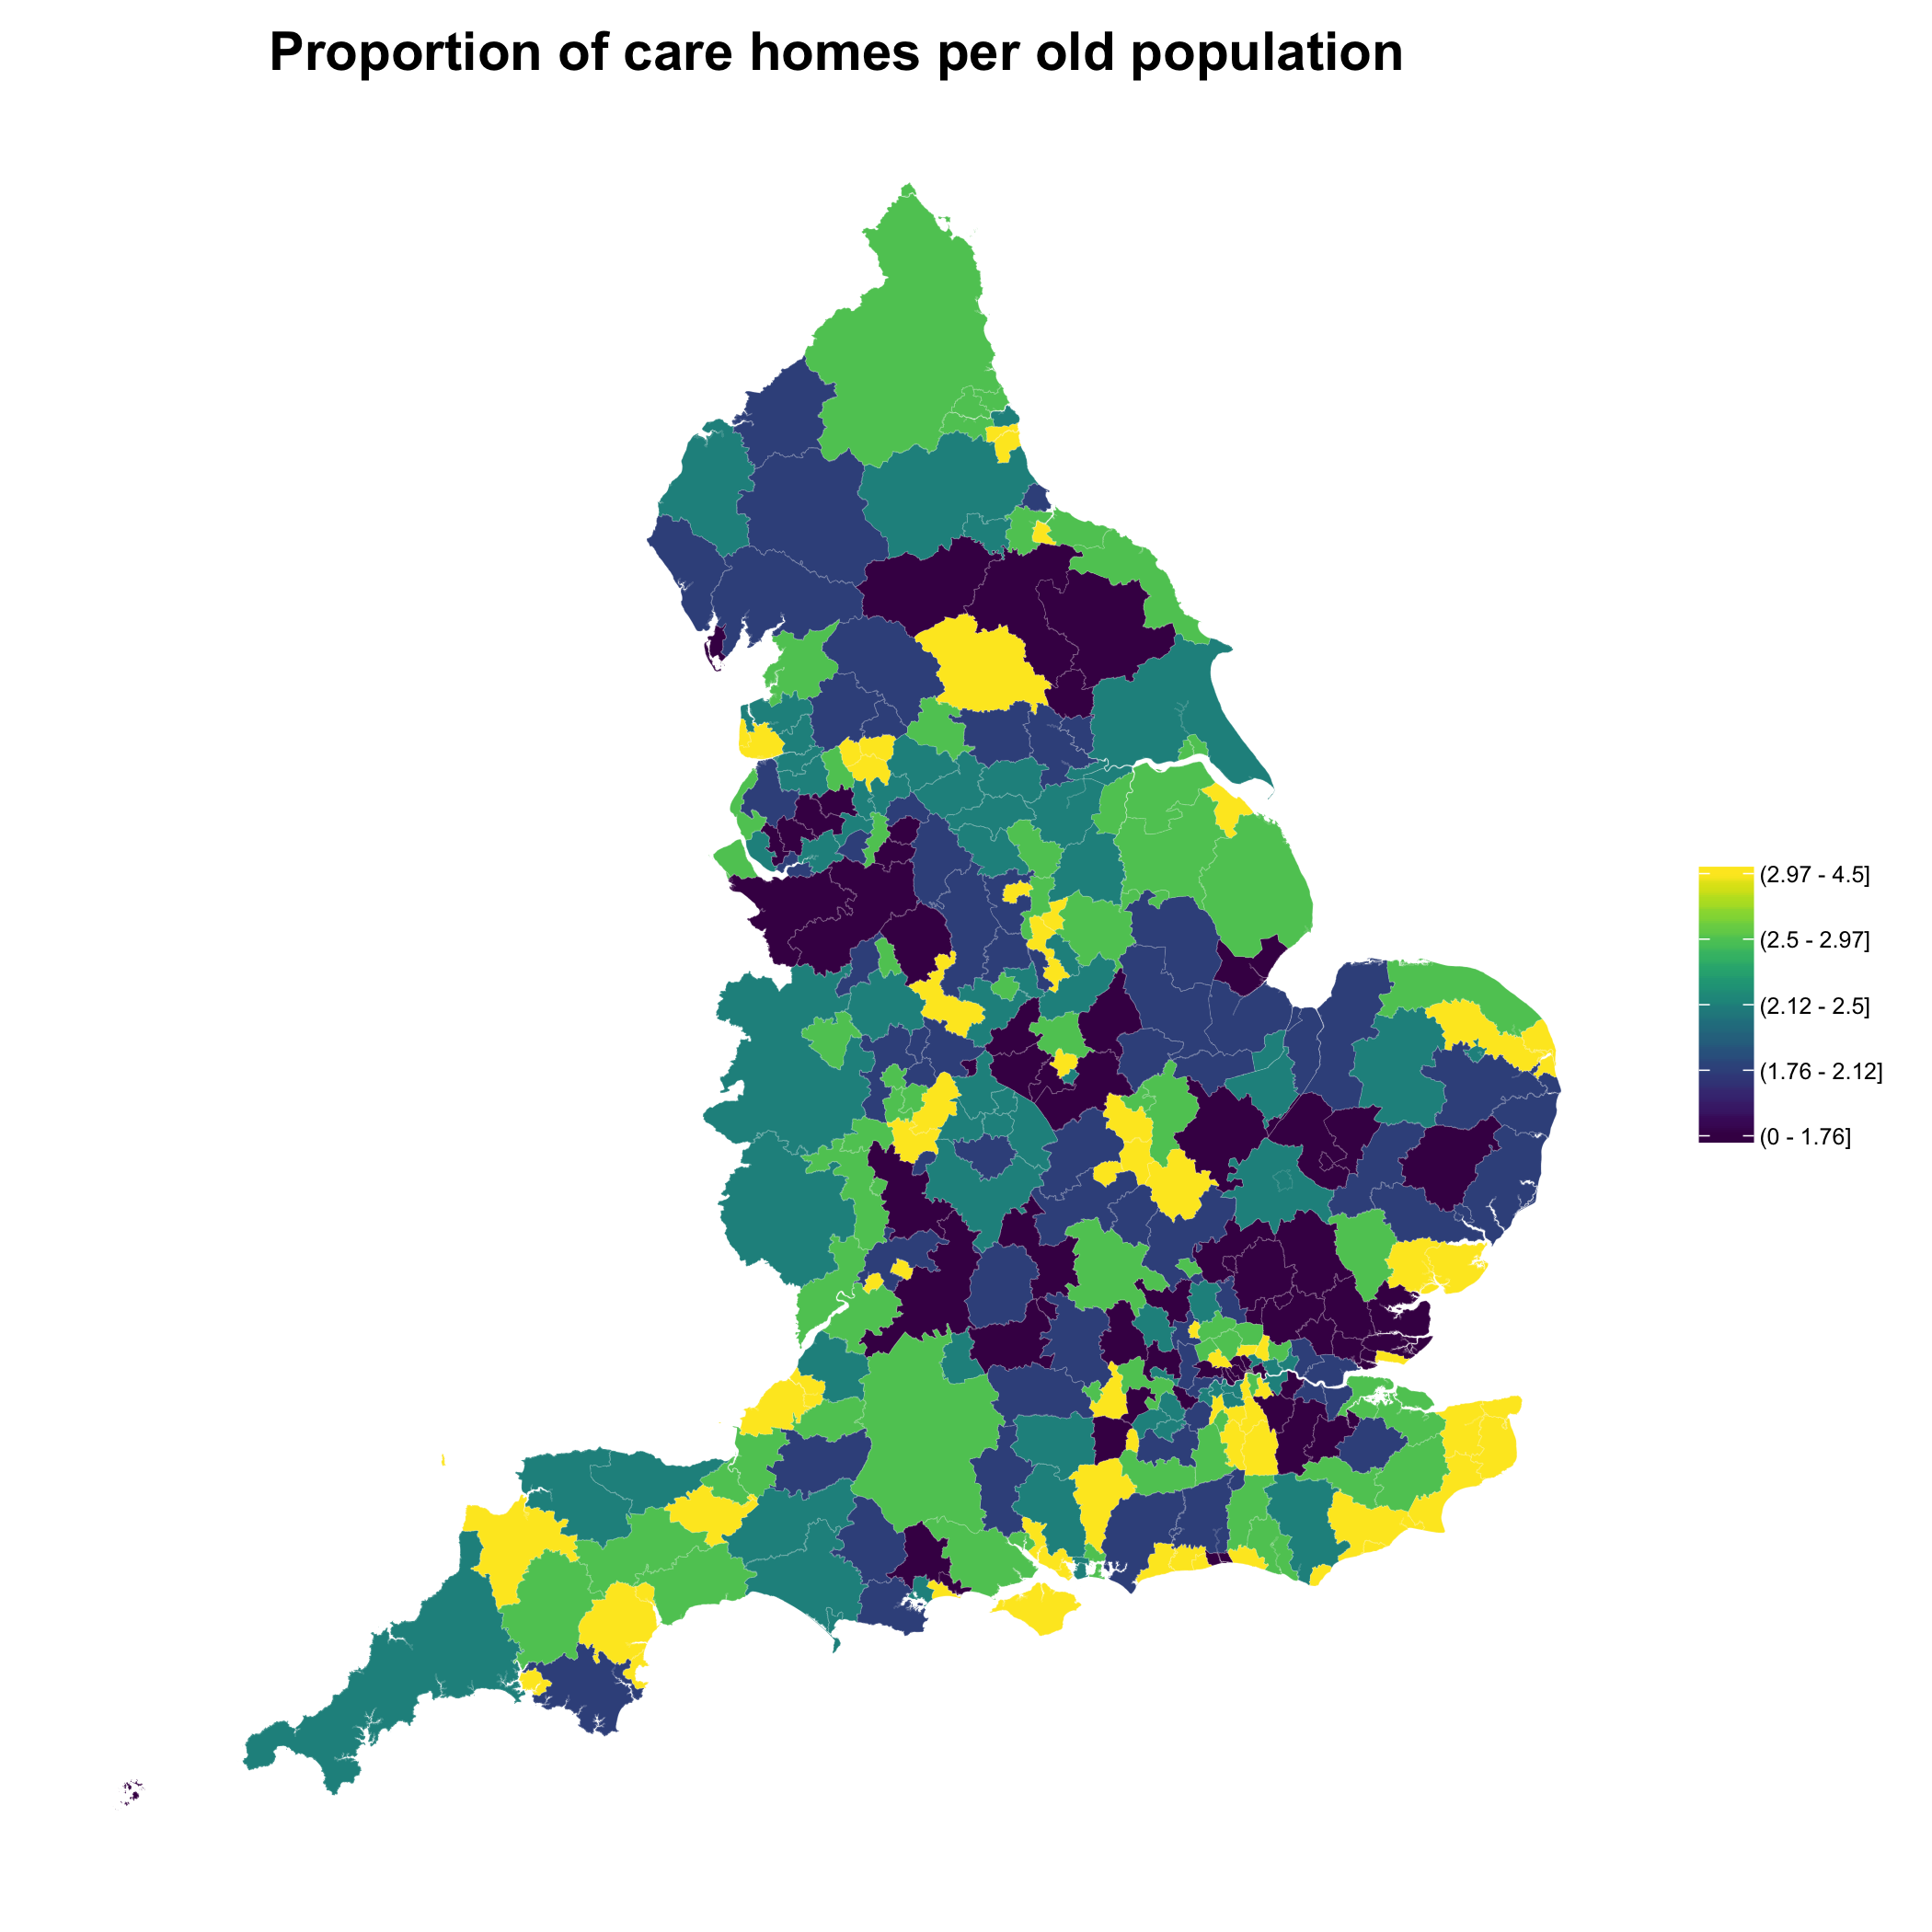
\includegraphics[width=1\textwidth]{ch_2/map_care_homes.png}


\floatfoot{{\textbf{Note}}: Aging}
\end{figure}


\newpage
\section{Tables}
\label{sec: tables}

\begin{table}[!h]
\caption{Your model here}
\label{tab: second_stage}
\resizebox{\textwidth}{!}{%
\begin{tabular}{@{}lccccccc@{}}
\toprule
                           & \multicolumn{3}{c}{Number of care homes per 1000 population 65+} & \multicolumn{1}{l}{} & \multicolumn{3}{c}{Entry rates}   \\ 
                     \cmidrule(r){2-4} \cmidrule(r){6-8} \\
 
                           & (1)                  & (2)                 & (3)                 &                    & (4)       & (5)       & (6)       \\
                          \cmidrule(r){2-4} \cmidrule(r){6-8} \\
Average house prices (log) & -0.780***            & -0.107              & -0.622***           &                      & -0.00385  & -0.0103** & -0.00652  \\
                           & (0.118)              & (0.0898)            & (0.178)             &                      & (0.00478) & (0.00406) & (0.00868) \\
\midrule\\
Estimation                 & OLS                  & IV                  & IV                  &                      & OLS       & IV        & IV        \\
Time FE                    &                      & Yes                 & Yes                 &                      &           & Yes       & Yes       \\
Region FE                  &                      & No                  & Yes                 &                      &           & No        & Yes       \\
\midrule
\\
Observations               & 1260                 & 1260                & 1260                &                      & 1260      & 1260      & 1260      \\
Local Authorities          & 315                  & 315                 & 315                 &                      & 315       & 315       & 315       \\
R-squared                  & 0.209                & 0.043               & 0.204               &                      & 0.021     & 0.014     & 0.048     \\ \bottomrule
\end{tabular}%
}
\begin{tablenotes}
     \scriptsize
      \item  {\textbf{Note}}: Your sources here.  
      Your explanation here . $^{***}p<0.01$,$^{**}p<0.05$, ${^*}p<0.1$ \end{tablenotes}
\end{table}